\documentclass[10pt,hyperref={CJKbookmarks=true},xcolor=dvipsnames,aspectratio=169]{beamer}
\usetheme[navigation]{UMONS}
\usepackage[utf8]{inputenc}
\usepackage{verbatim}
\usepackage{ctex}

\title[国际经济学]{国际经济学}
\subtitle{全球贸易典型事实与贸易量的决定}
\author{鲁晓东}
\institute[]{%
	岭南学院\hspace{2em}中山大学
	\\[4ex]
	
\includegraphics[height=8ex]{fig/lingnanlogo}\hspace{2em}%
	
\includegraphics[height=8.5ex]{fig/sysu}
}
%------------section前展示一页----------
\AtBeginSection[] {     
	\begin{frame}        
	\tableofcontents[currentsection,hideallsubsections]    
\end{frame} 
}

%-------------subsection也展示一下----------
\AtBeginSubsection[]{
	
	\frame<beamer>{ 
		
		\frametitle{Outline}   
		
		\tableofcontents[currentsection,currentsubsection] 
		
	}
	
}
%---------------------------

%-----------一段一闪现-------
%\beamerdefaultoverlayspecification{<+->}
%这个功能基本不用

\begin{document}
	\maketitle
	
	
	\begin{frame}
	\frametitle{提纲}
	\tableofcontents
\end{frame}				%生成提纲页

%-----------正文开始----------------------



\section{Stylized Facts about World Economy}%

\subsection[全球贸易]{Global Trade}
 

\begin{frame}{全球贸易大图景(1500-20111)}
 \begin{columns}[onlytextwidth]
 	\begin{column}{0.4\textwidth}
 			\begin{itemize}
 				\item 过去五个世纪,全球贸易的role与日俱增
 				\item 这种趋势是否还会延续(glob or deglob?)
 			\end{itemize}
 	\end{column}
 	
 	
 	\begin{column}{0.6\textwidth}
 		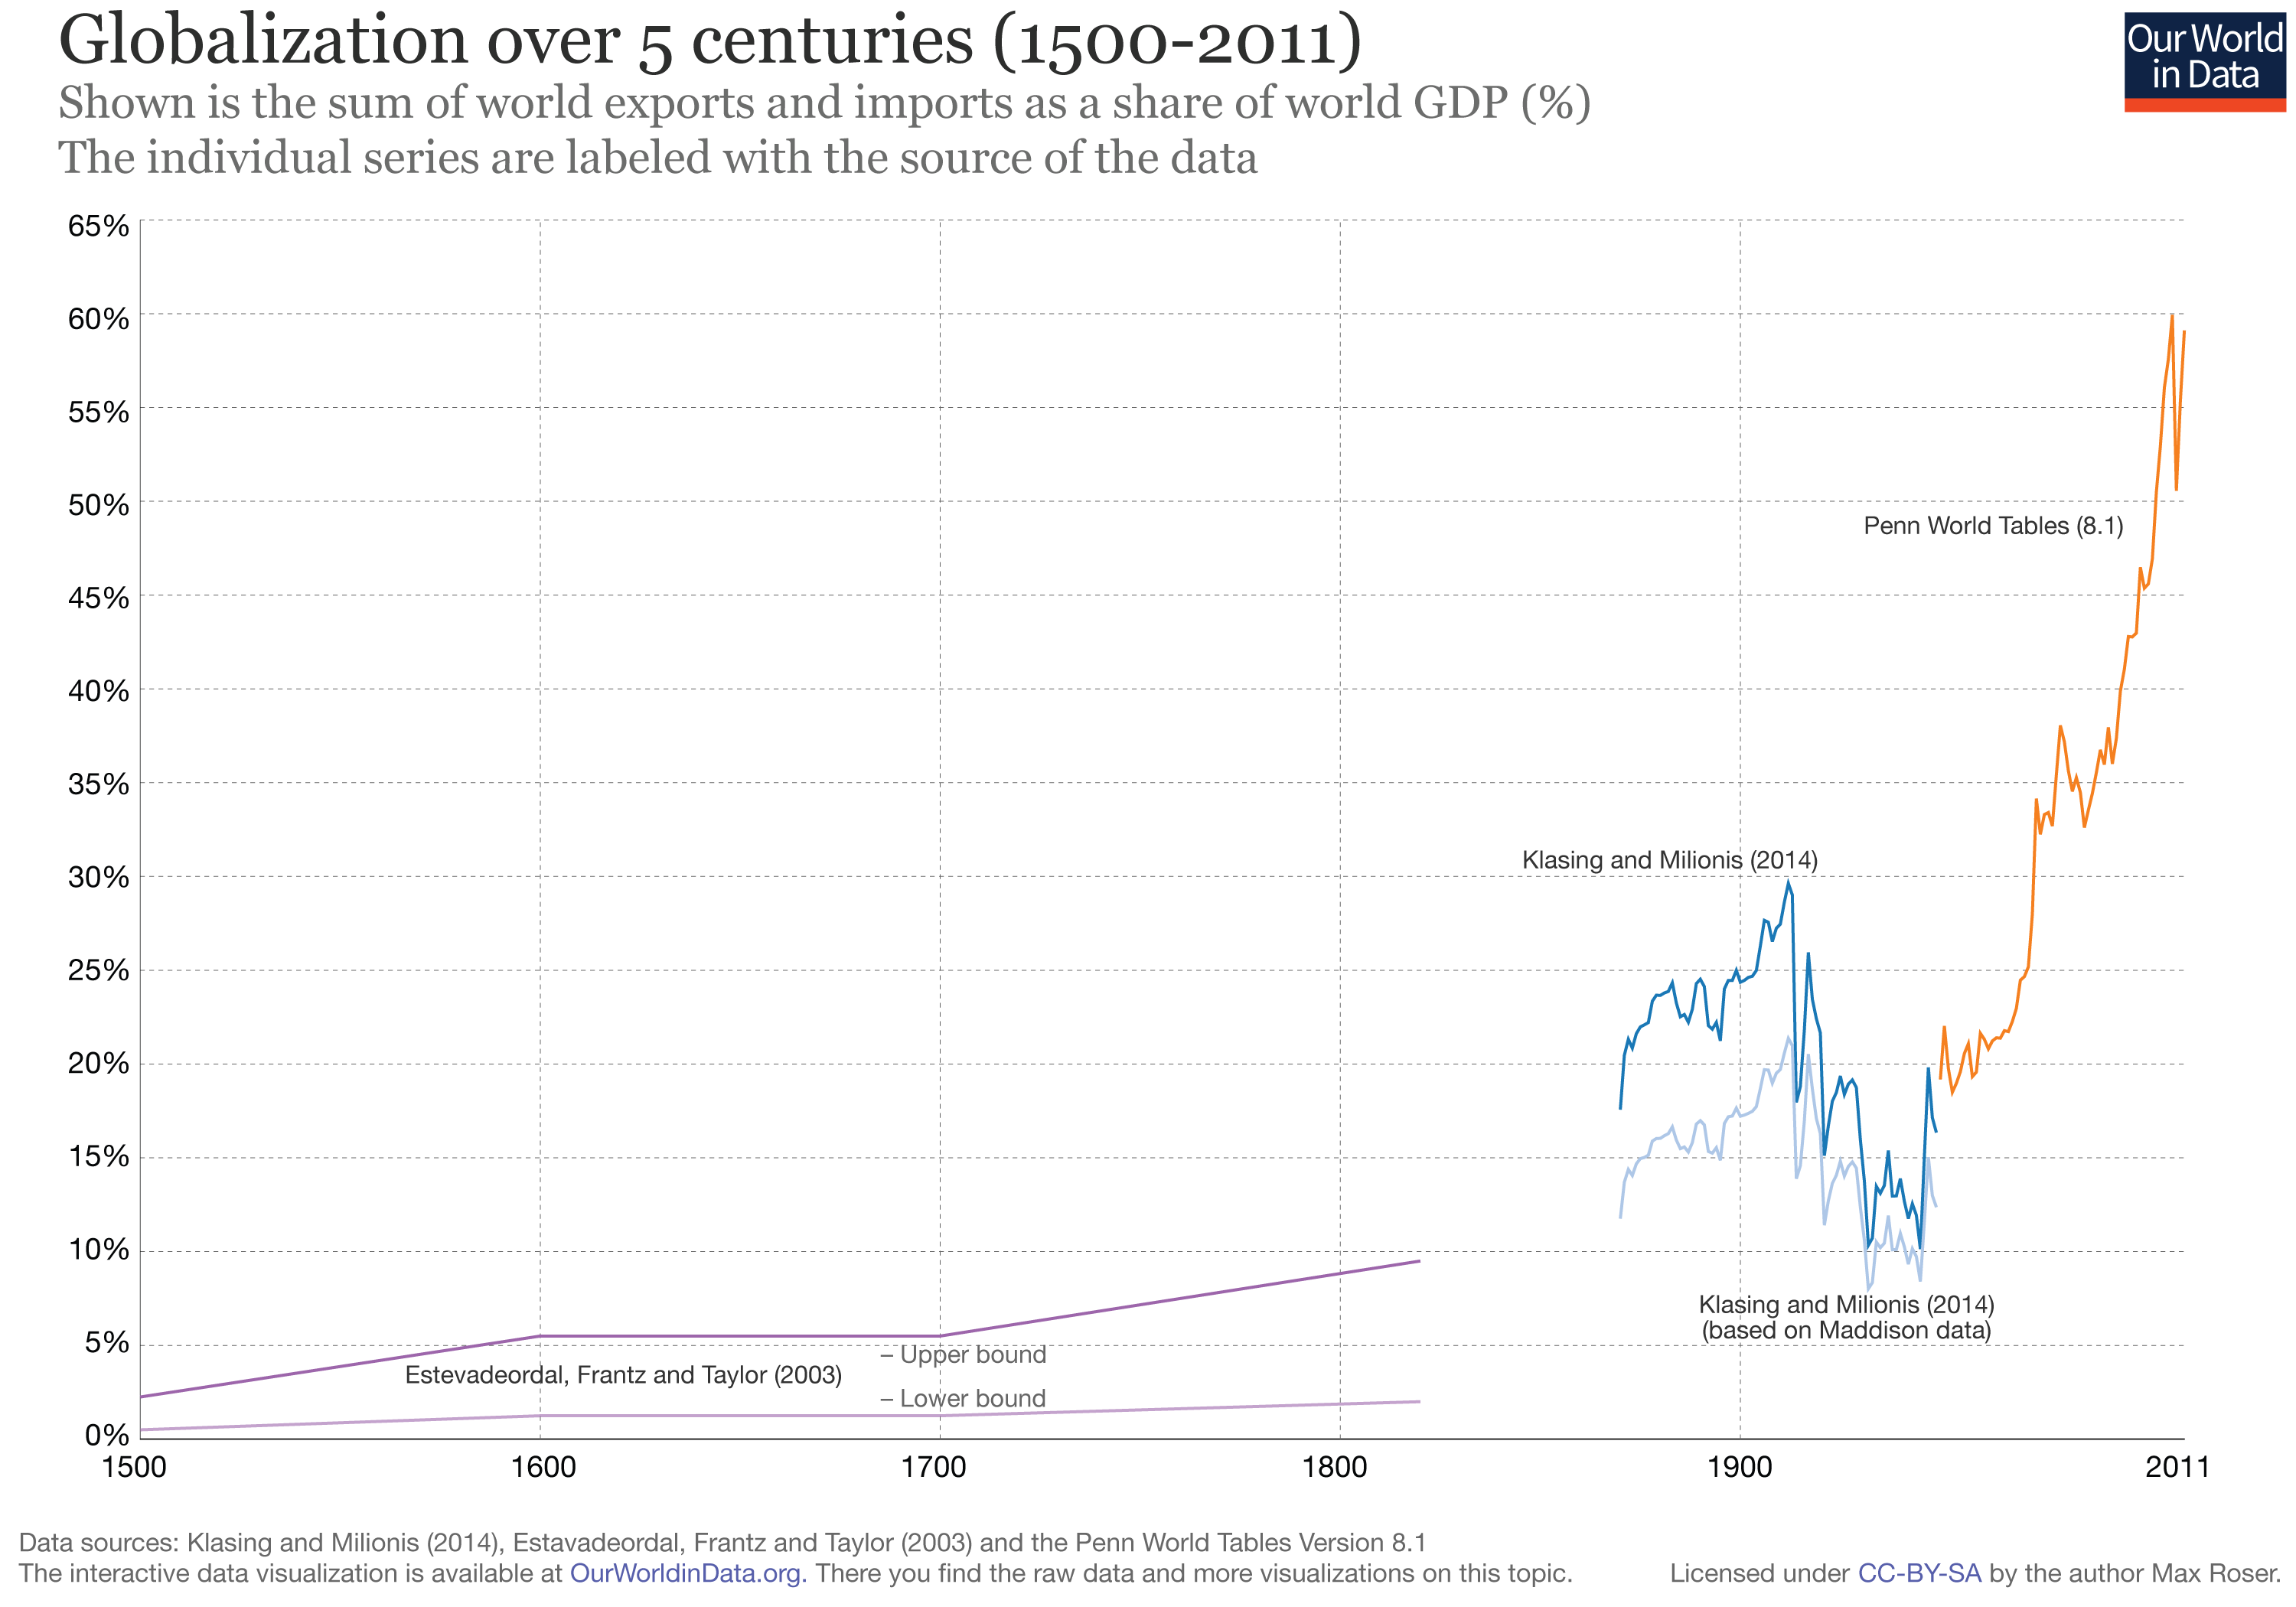
\includegraphics[scale=0.1]{fig/gravity/ourworldindata_world-trade-over-5-centuries}
 	\end{column}
 	
 \end{columns}	

\end{frame}

\begin{frame}{全球化的三次浪潮}
\centering 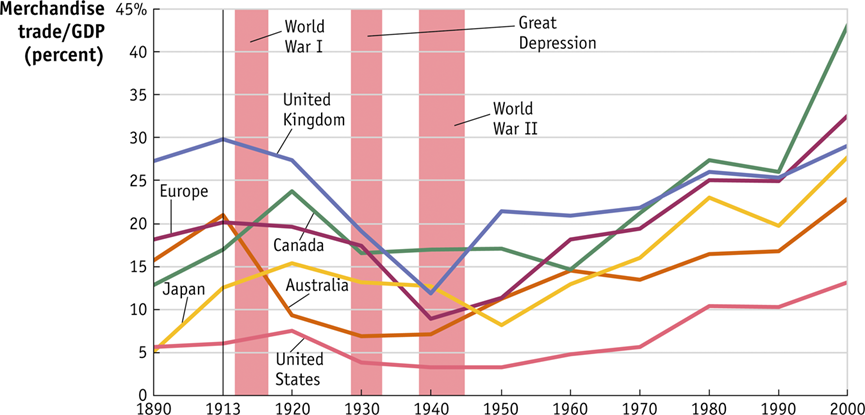
\includegraphics[scale=0.7,]{fig/gravity/glo3}
\end{frame}


\begin{frame}{谁在参与贸易}
\centering 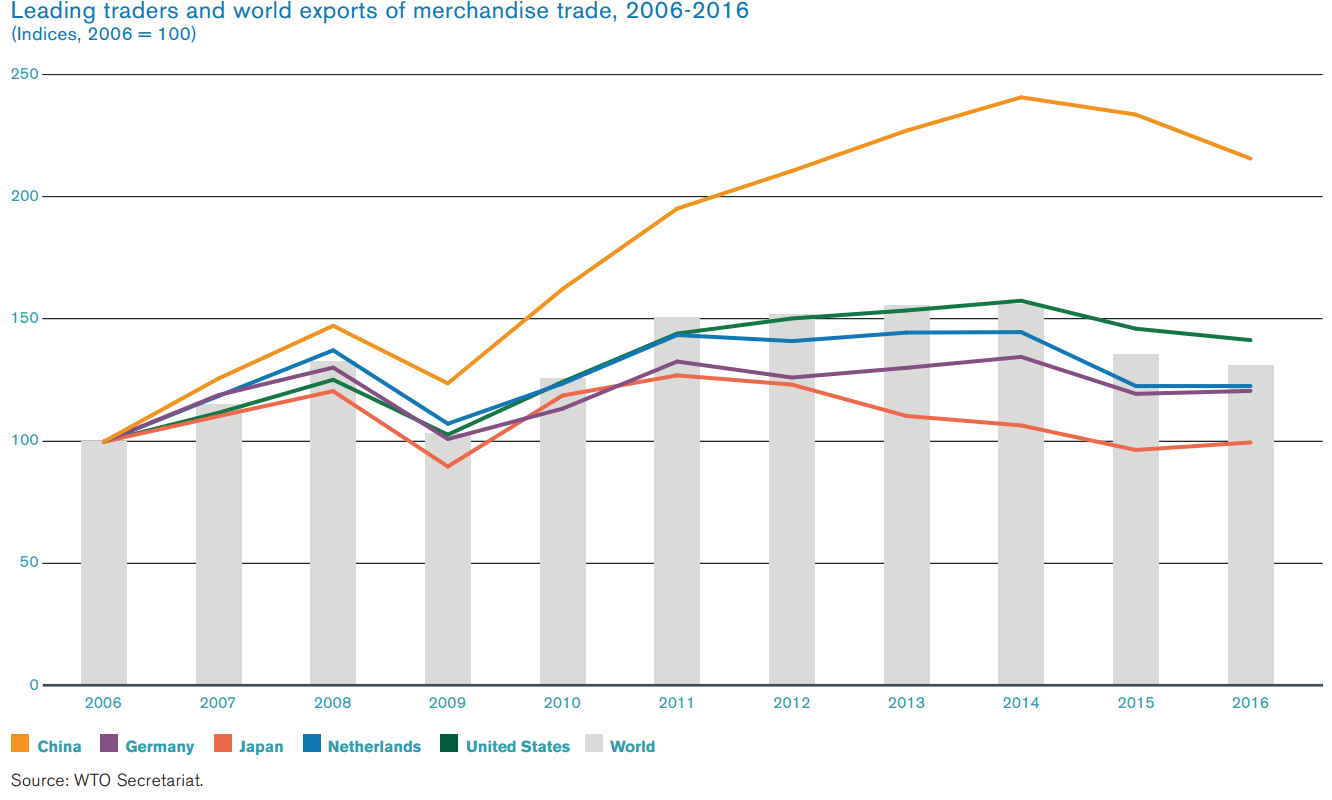
\includegraphics[scale=0.35]{fig/gravity/leadingtraders}
\end{frame}


\begin{frame}{全球主要经济体贸易依存度}
\centering 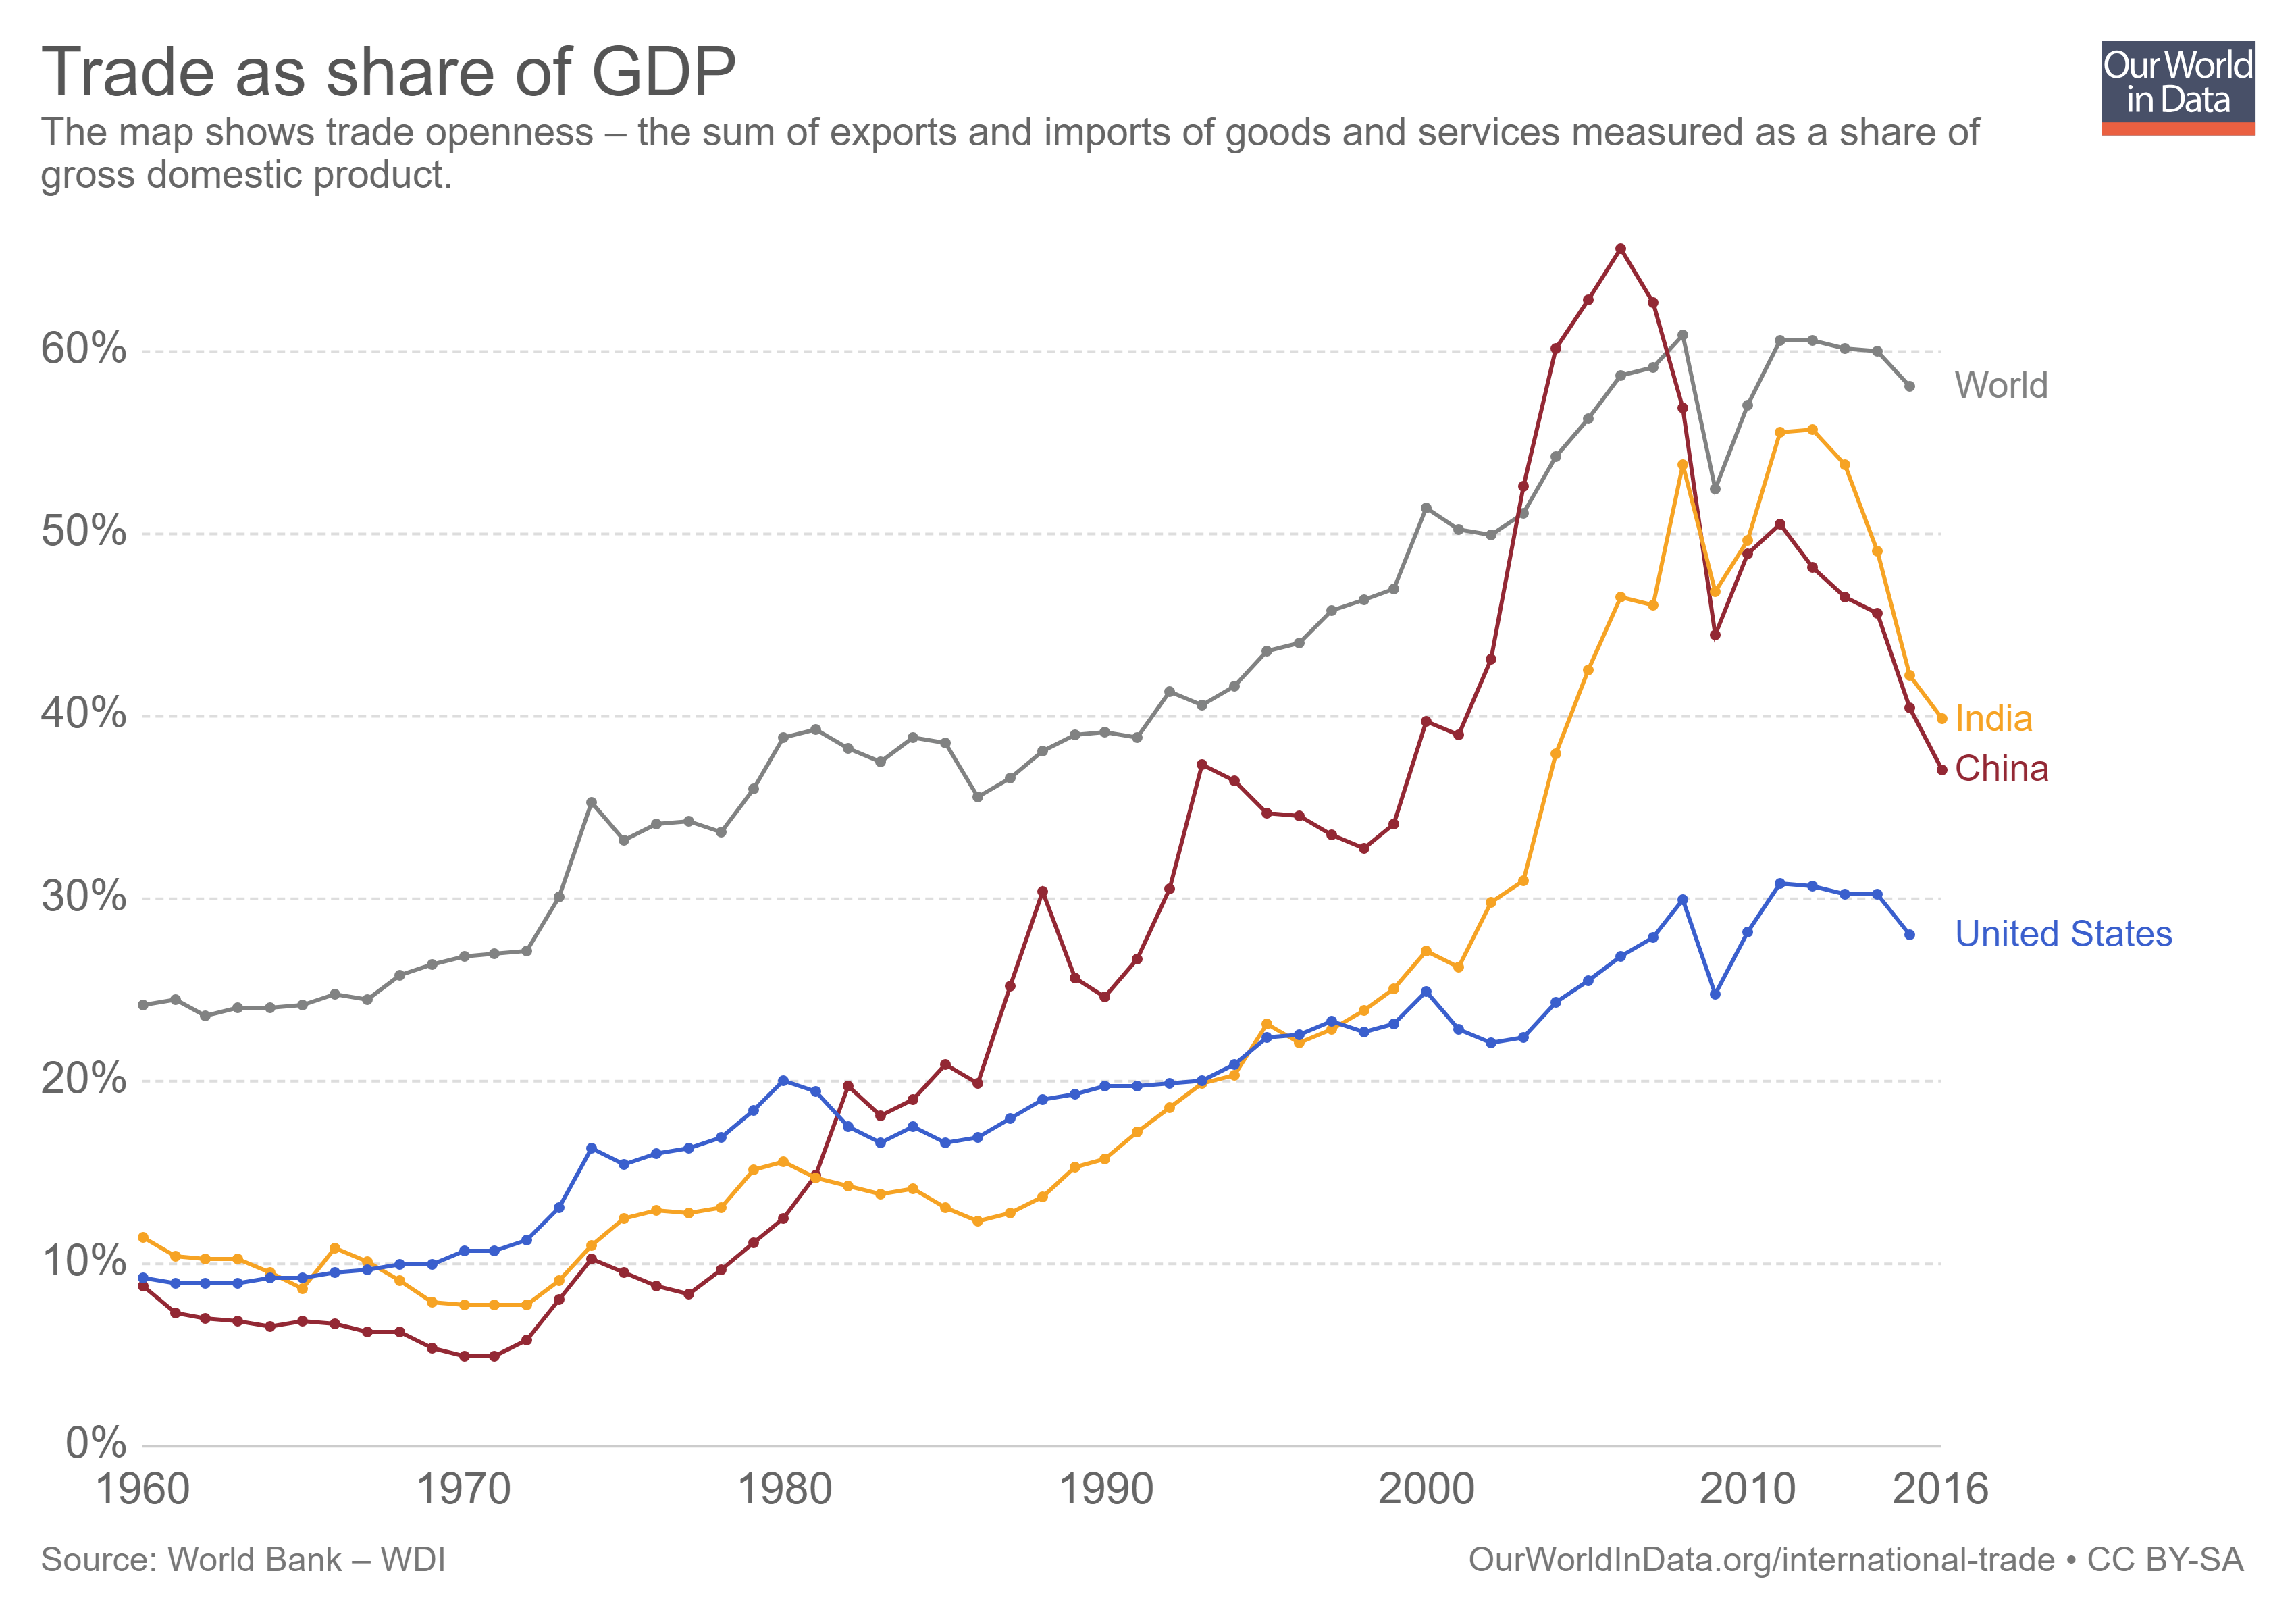
\includegraphics[scale=0.08]{fig/gravity/trade-as-share-of-gdp}
\end{frame}


\subsection[贸易的产品结构]{What does the world trade?}



\begin{frame}
\begin{itemize}
	\item Mostly manufactures 
	\item Trade in services is growing as a share of world trade 
	\begin{figure}
		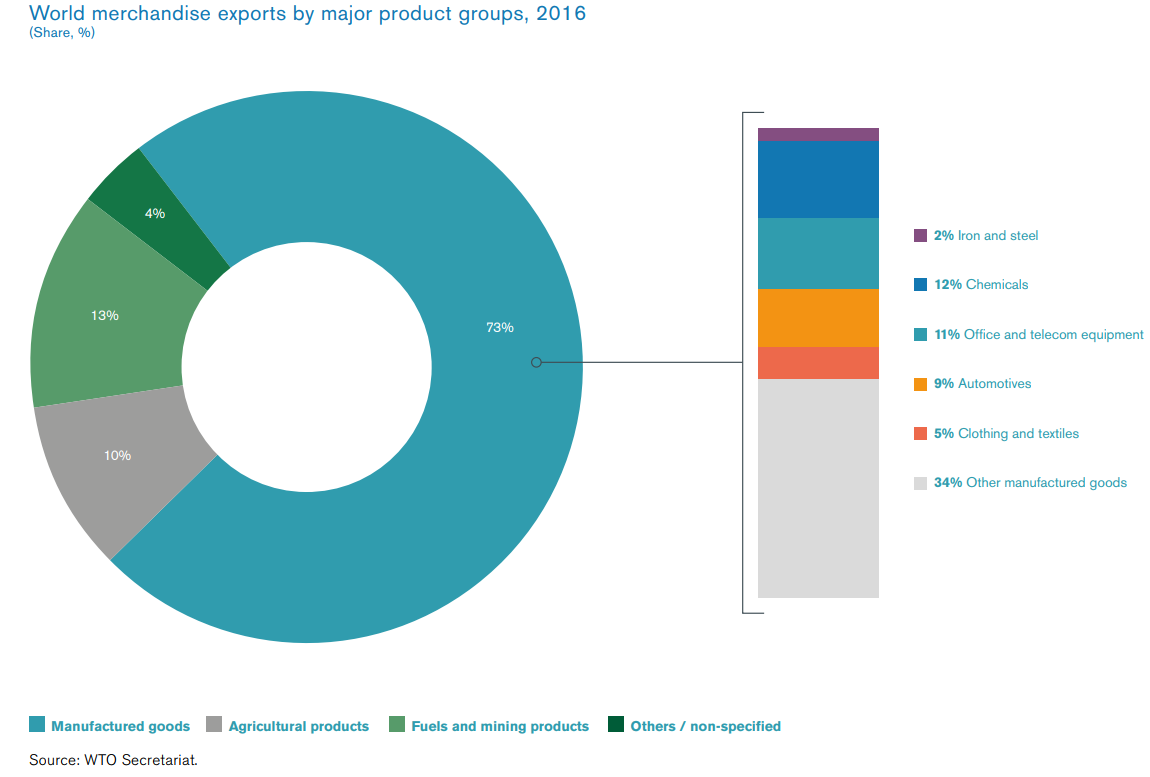
\includegraphics[scale=0.3]{fig/gravity/tra1}
		
	\end{figure}
	
\end{itemize}
\end{frame}

\begin{frame}{What Does the World Trade?}

\begin{itemize}
\item Fuel and mining products are key exports for some countries
\begin{figure}
	\begin{centering}
		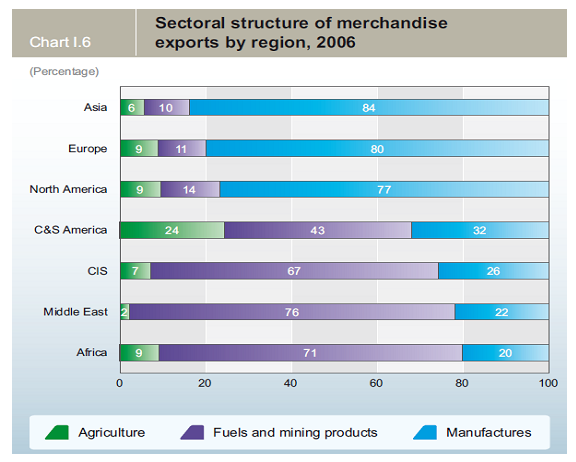
\includegraphics[width=7cm]{fig/gravity/tra2}
		\par\end{centering}
	
\end{figure}

\end{itemize}
\end{frame}

\begin{frame}{What is traded around the world}
\centering	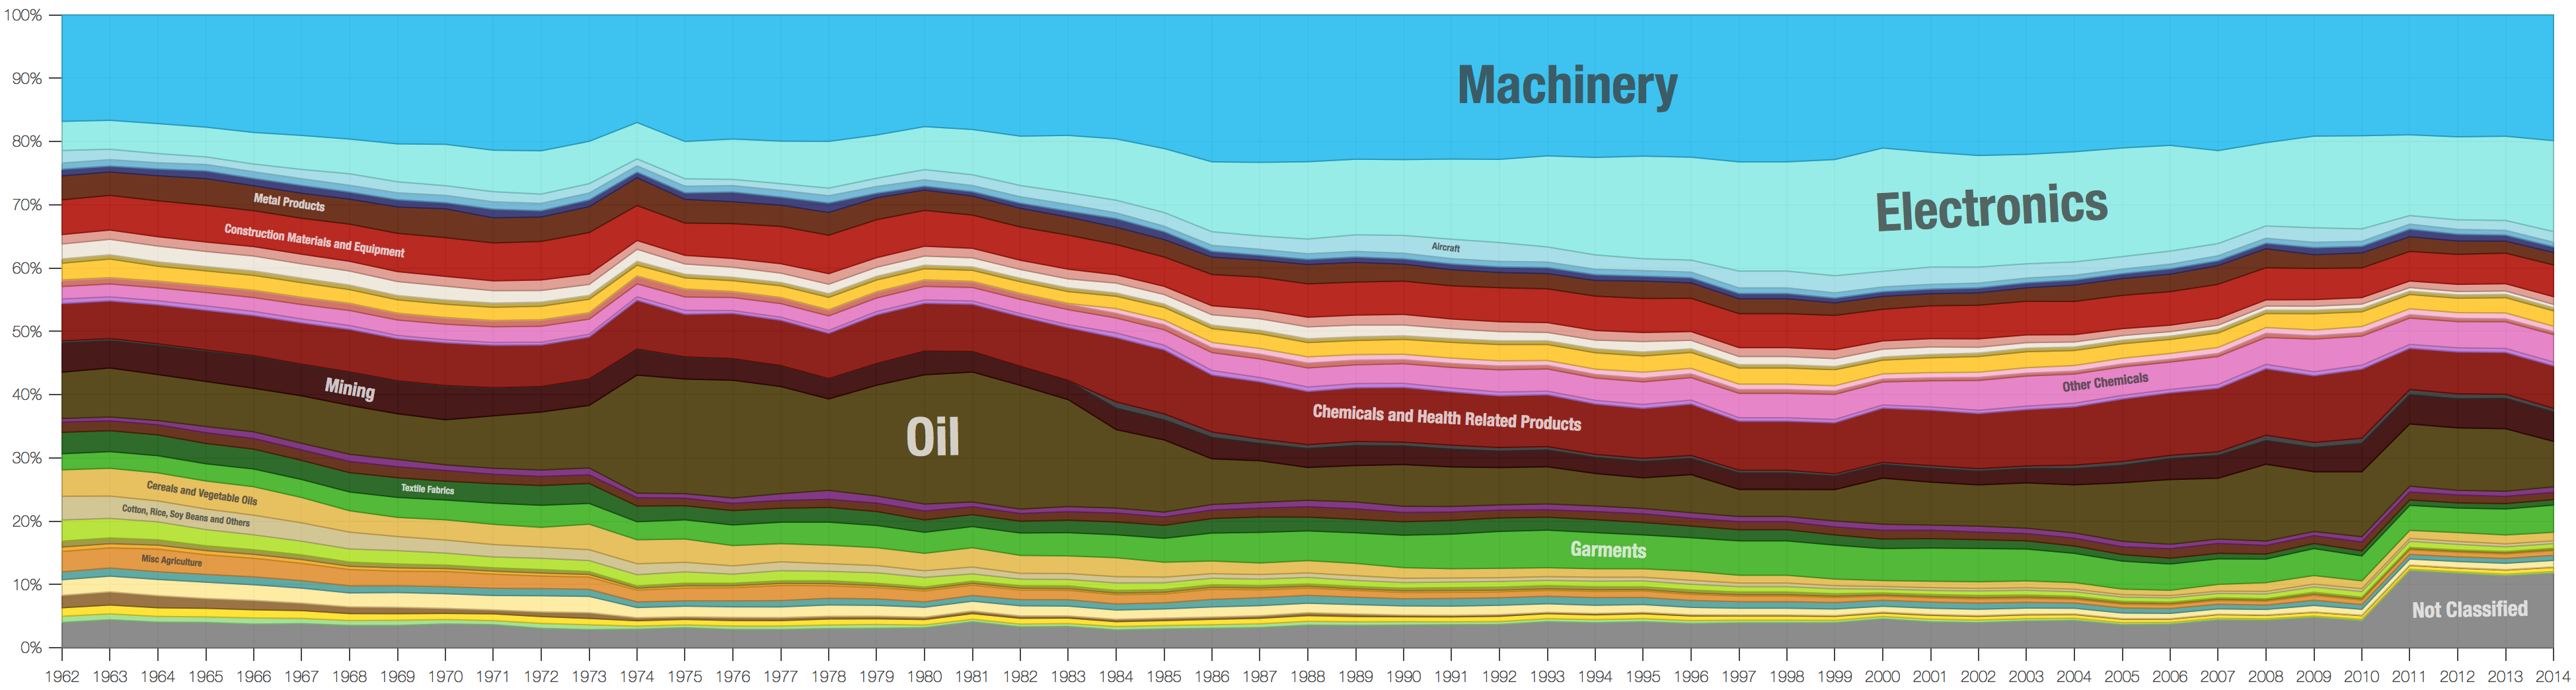
\includegraphics[scale=0.24]{fig/gravity/OEC_Trade_Products}
\end{frame}

\begin{frame}{What Did XXX Export in 2013?}


\begin{figure}


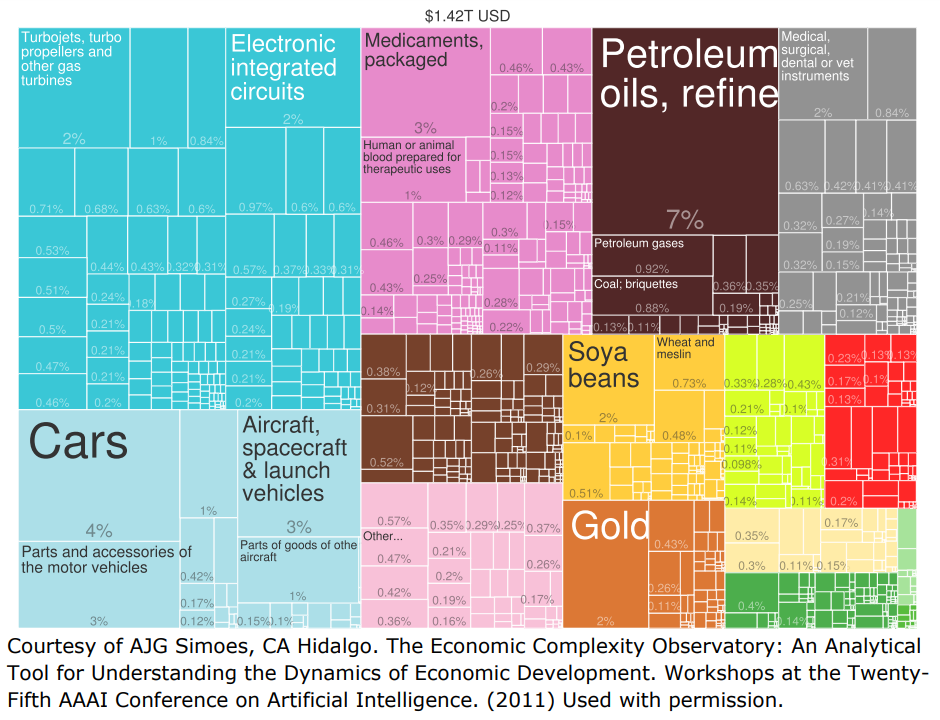
\includegraphics[scale=0.35]{fig/gravity/com2-1.PNG}

\end{figure}

\end{frame}

\begin{frame}{What Did U.S. Export in 2013?}


\begin{figure}
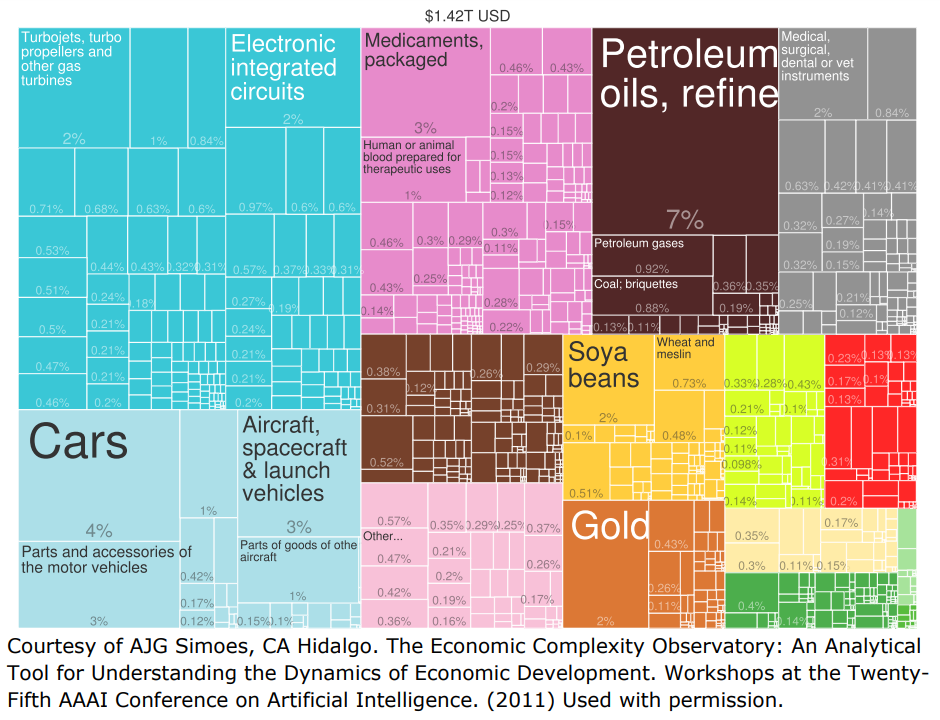
\includegraphics[scale=0.35]{fig/gravity/com2-1.PNG}
\end{figure}

\end{frame}

\begin{frame}{What Did XXX Export in 2013?}


\begin{figure}
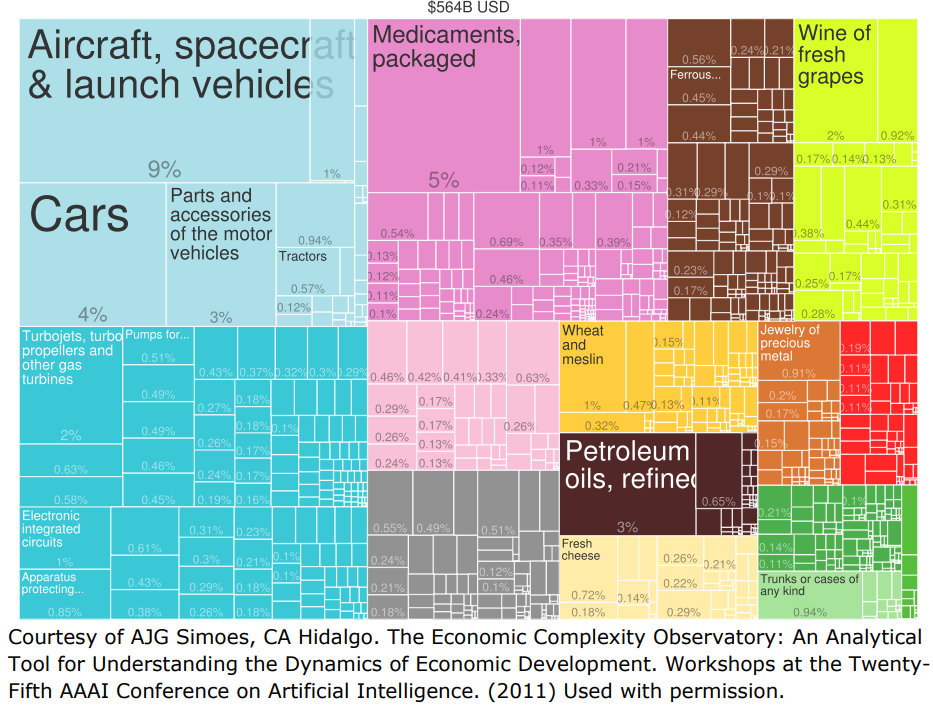
\includegraphics[scale=0.35]{fig/gravity/com2-2.PNG}
\end{figure}

\end{frame}

\begin{frame}{What Did France Export in 2013?}


\begin{figure}
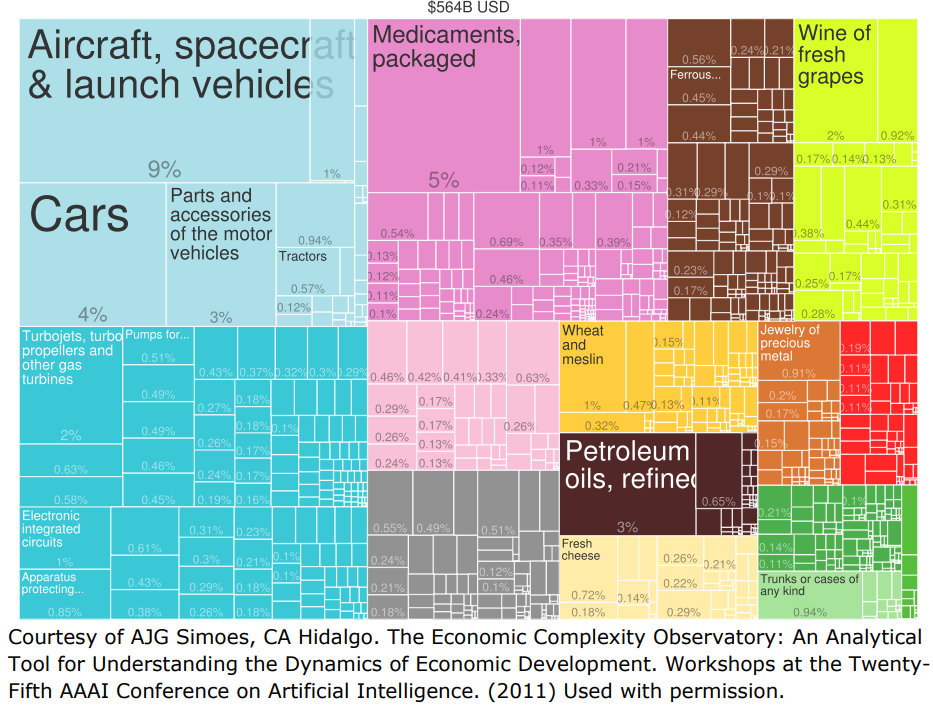
\includegraphics[scale=0.35]{fig/gravity/com2-2.PNG}
\end{figure}

\end{frame}

\begin{frame}{What Did XXX Export in 2013?}


\begin{figure}
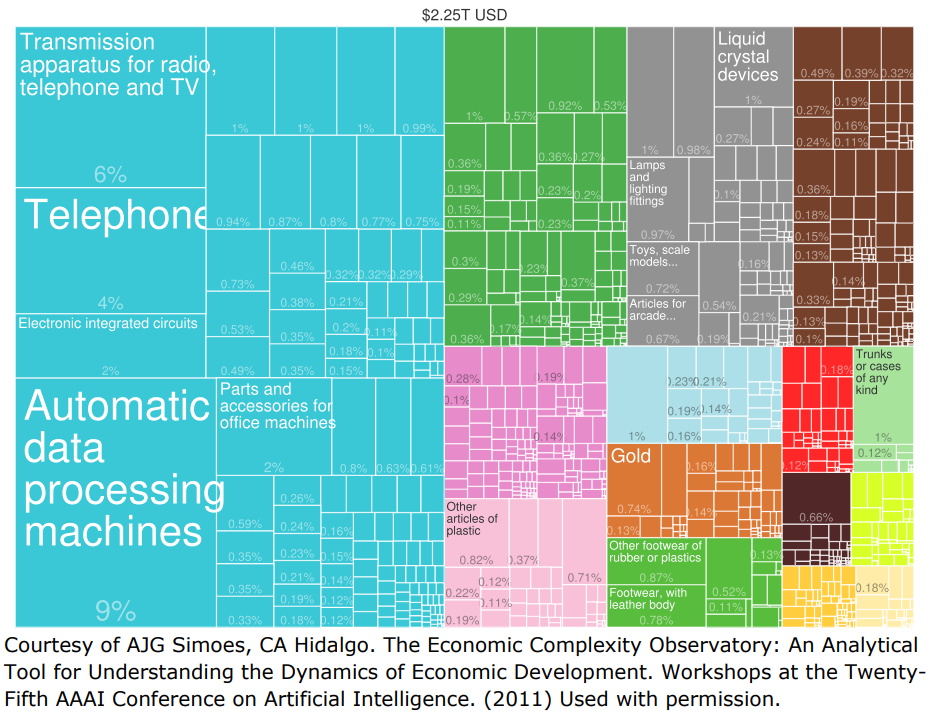
\includegraphics[scale=0.35]{fig/gravity/com2-3.PNG}
\end{figure}

\end{frame}

\begin{frame}{What Did China Export in 2013?}


\begin{figure}
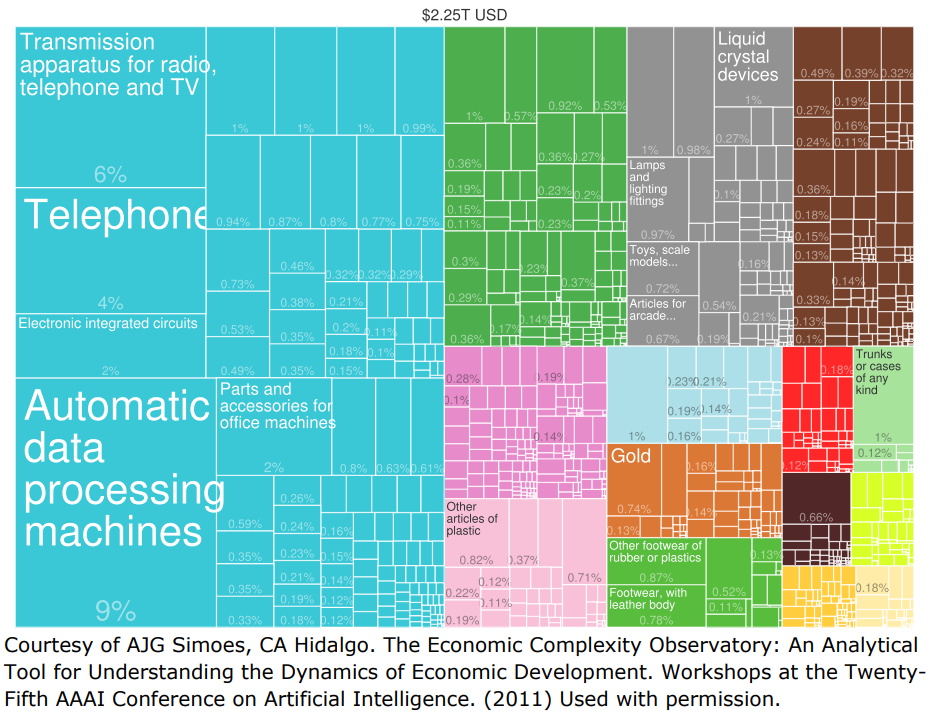
\includegraphics[scale=0.35]{fig/gravity/com2-3.PNG}
\end{figure}

\end{frame}

\begin{frame}{What Did XXX Export in 2013?}


\begin{figure}
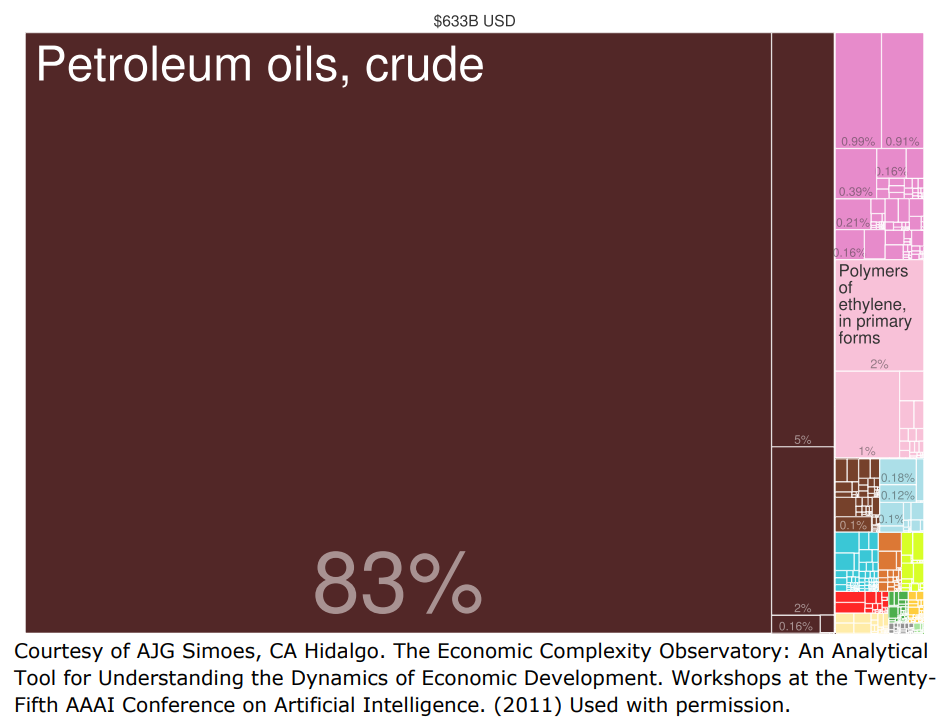
\includegraphics[scale=0.35]{fig/gravity/com2-4.PNG}
\end{figure}

\end{frame}

\begin{frame}{What Did Saudi Arabia Export in 2013?}


\begin{figure}
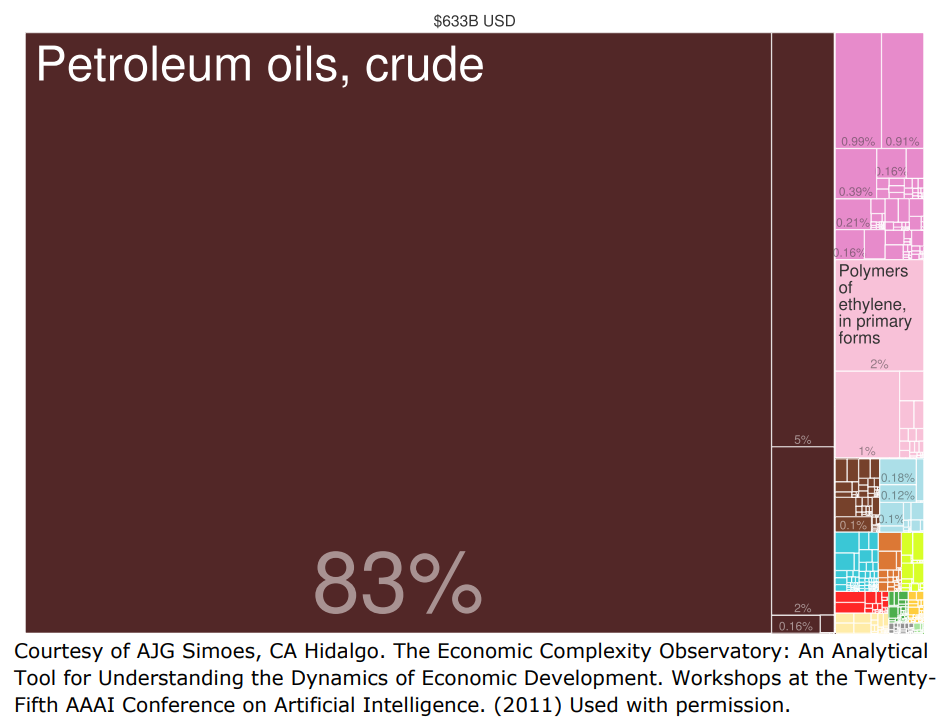
\includegraphics[scale=0.35]{fig/gravity/com2-4.PNG}
\end{figure}

\end{frame}

\begin{frame}{What Did XXX Export in 2013?}


\begin{figure}
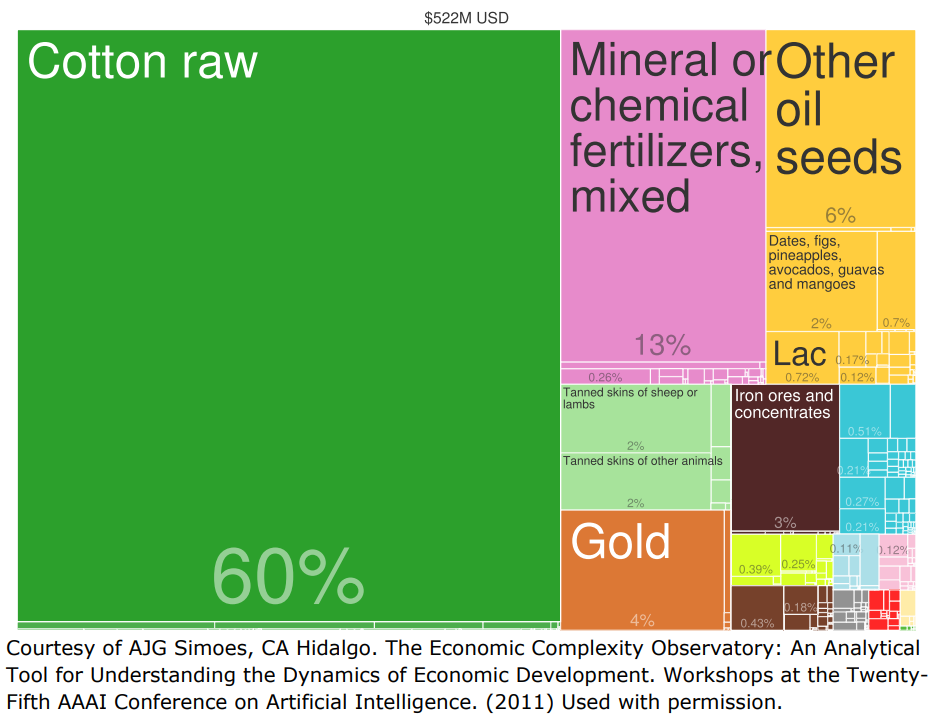
\includegraphics[scale=0.35]{fig/gravity/com2-5.PNG}
\end{figure}

\end{frame}

\begin{frame}{What Did Mali Export in 2013?}


\begin{figure}
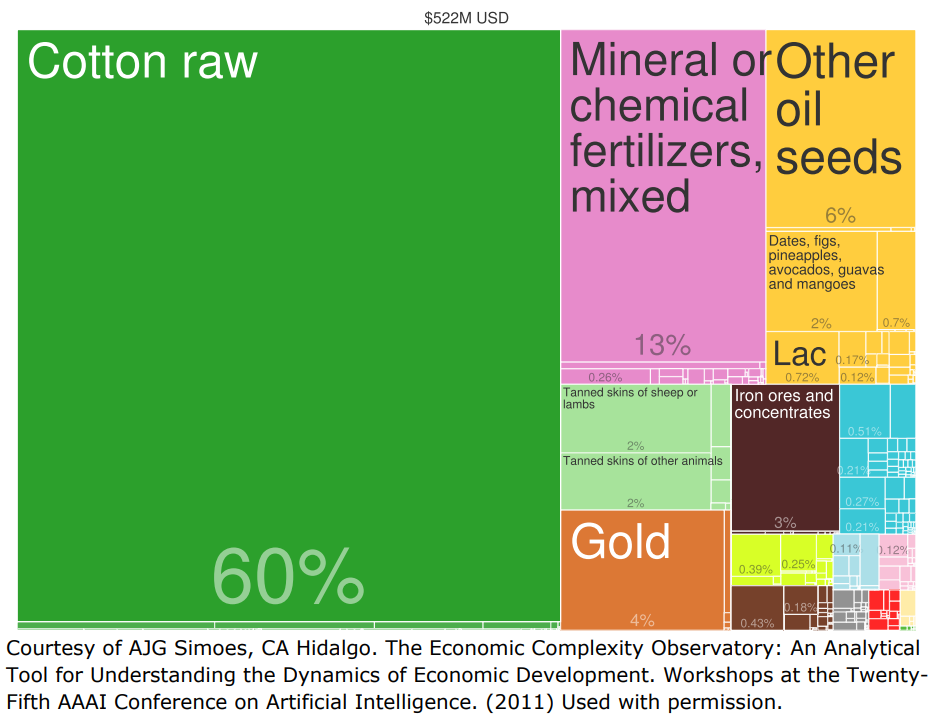
\includegraphics[scale=0.35]{fig/gravity/com2-5.PNG}
\end{figure}

\end{frame}

\begin{frame}{Export Composition of LDCs}


\begin{columns}[onlytextwidth]
\begin{column}{0.55\textwidth}
\begin{itemize}
\item Developing countries have substantially changed the composition of
their exports 
\item In 1960, 58\% of exports were agricultural products; 12\% manufactured
products 
\item In 2001, 65\% of exports were manufactured products; 10\% agricultural
products 
\end{itemize}

\end{column}
\begin{column}{0.45\textwidth}
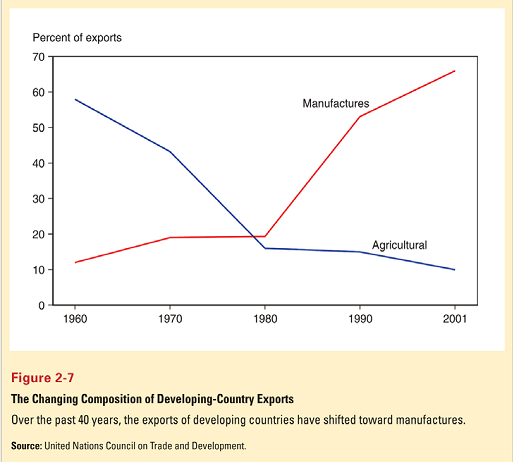
\includegraphics[width=\columnwidth]{fig/gravity/tra3}
\end{column}
\end{columns}

\end{frame}

\begin{frame}{Also True in Historical Perspective}


\begin{figure}


\begin{centering}
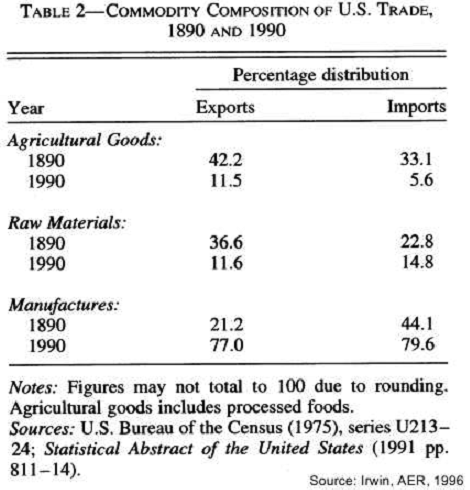
\includegraphics[width=6.5cm]{fig/gravity/tra4}
\par\end{centering}

\end{figure}

\end{frame}
\subsection[贸易的国别结构]{Who trade with whom?}

\begin{frame}{Who Trades with Whom?}

\begin{itemize}
	\item as a share of world merchandise trade, South–South trade more than tripled over 1980–2011, while North–North trade declined.
	\item China has been a key driver of this dynamic 
\end{itemize}

\begin{figure}
	
	
	\begin{centering}
		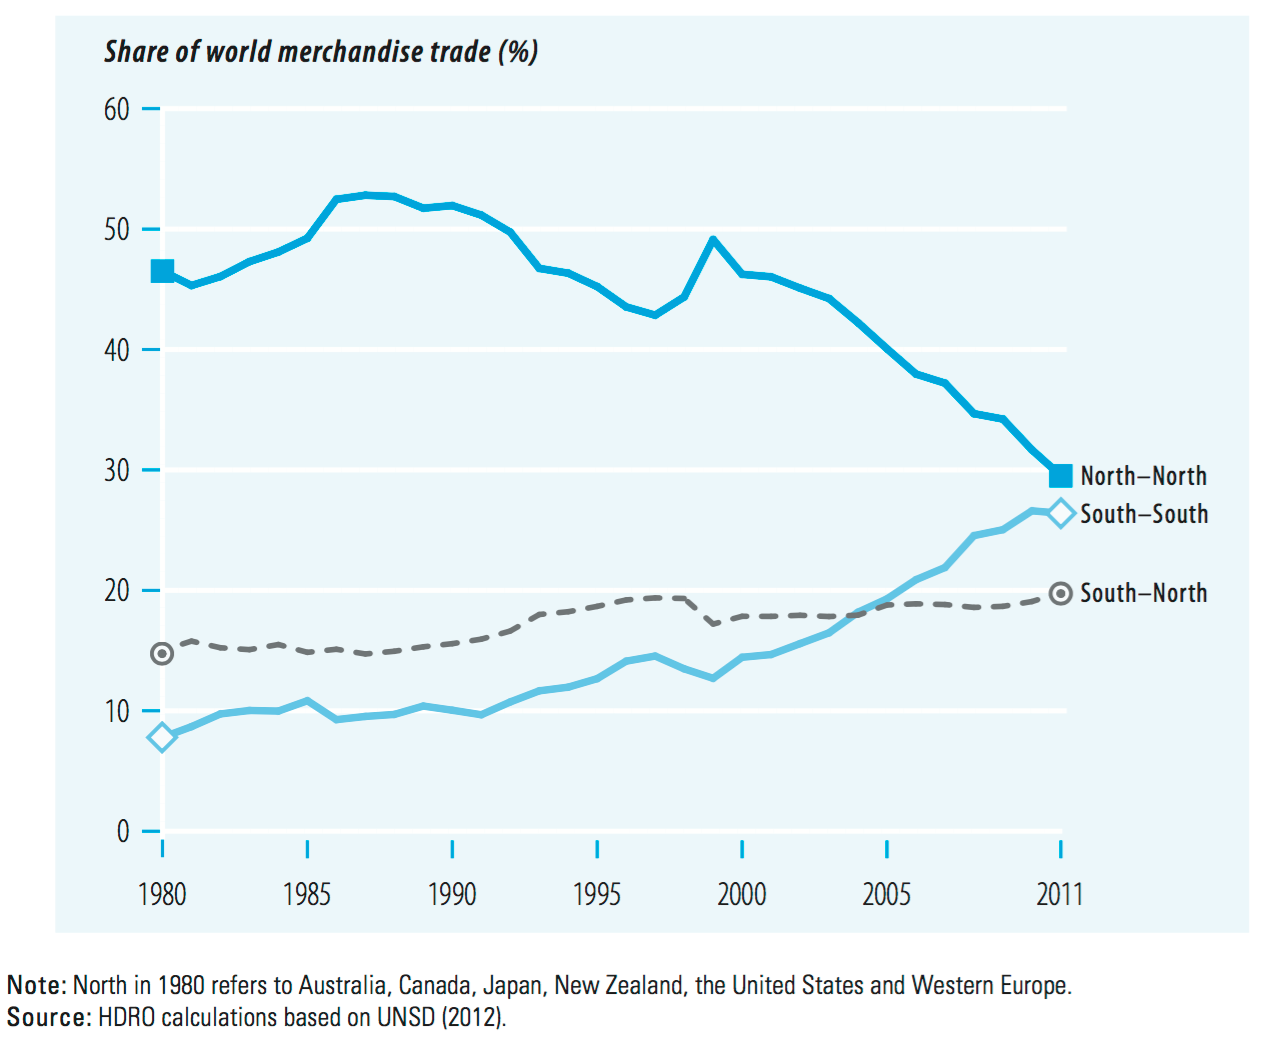
\includegraphics[width=8cm]{fig/gravity/SouthSouth_HDR2013}
		\par\end{centering}
	
\end{figure}


\end{frame}

\begin{frame}{认识一下全球贸易中的leaders}
\centering 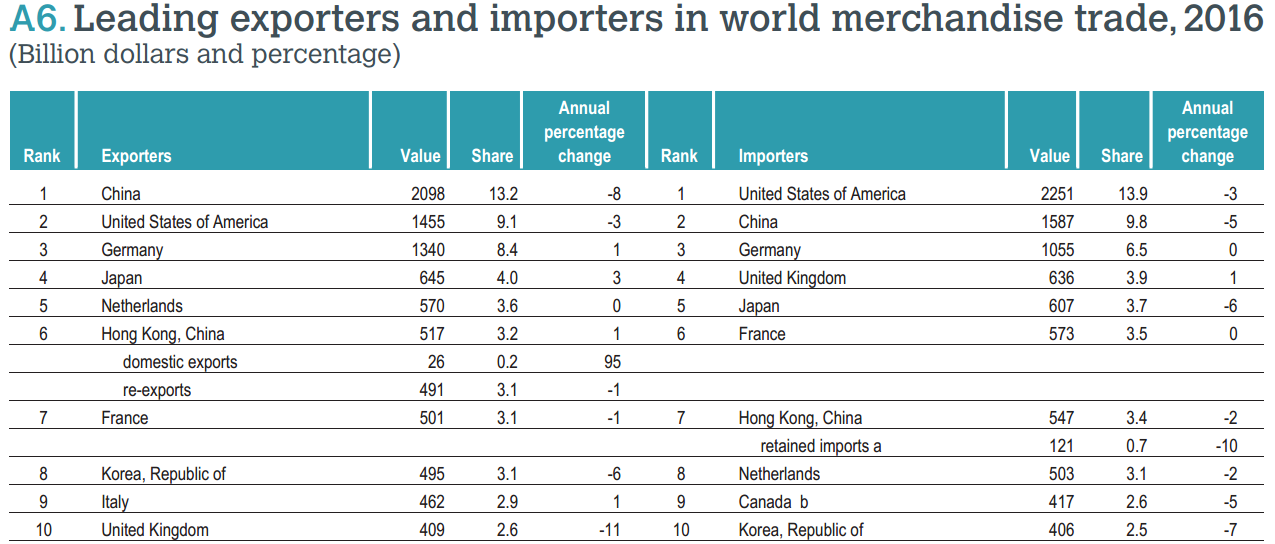
\includegraphics[scale=0.55]{fig/gravity/leaders}
\end{frame}



\subsection[中国在全球贸易中的角色]{the role of China in the world economy}

\begin{frame}{世界经济中的中国}
\centering 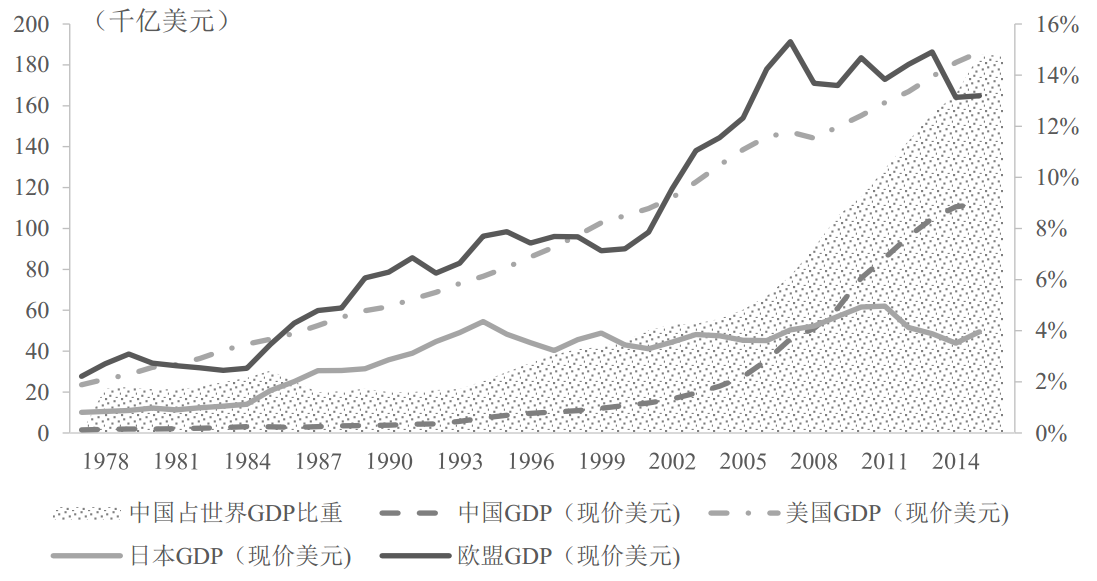
\includegraphics[scale=0.55]{fig/gravity/china0}
\end{frame}

\begin{frame}{世界贸易中的中国)}
\centering 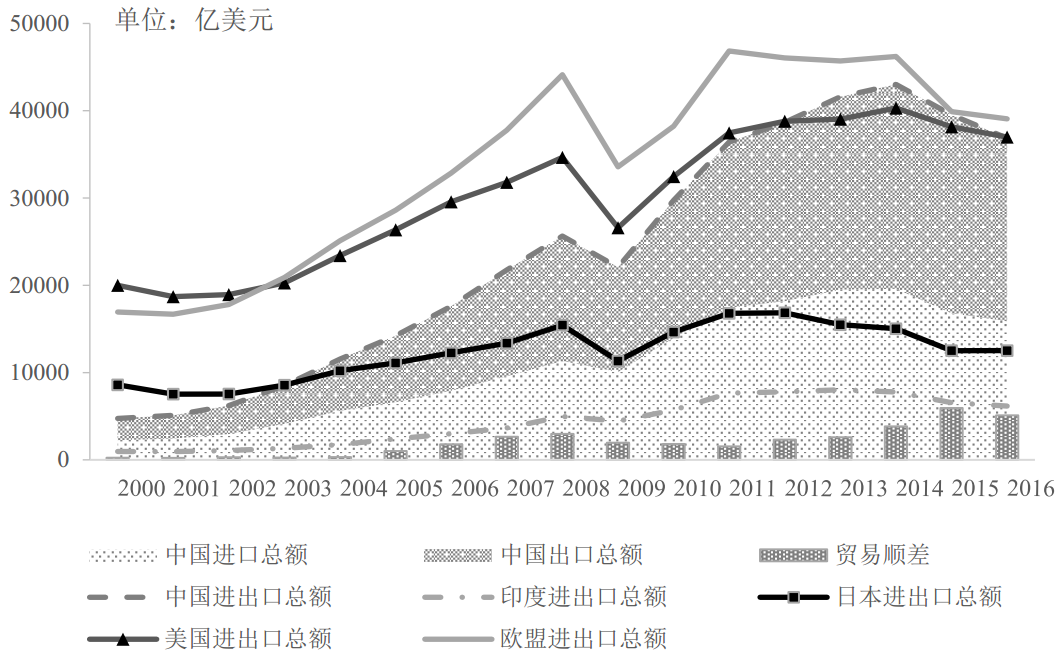
\includegraphics[scale=0.5]{fig/gravity/china1}
\end{frame}

\begin{frame}{中国进出口结构的变化(1980-2016 }
\centering 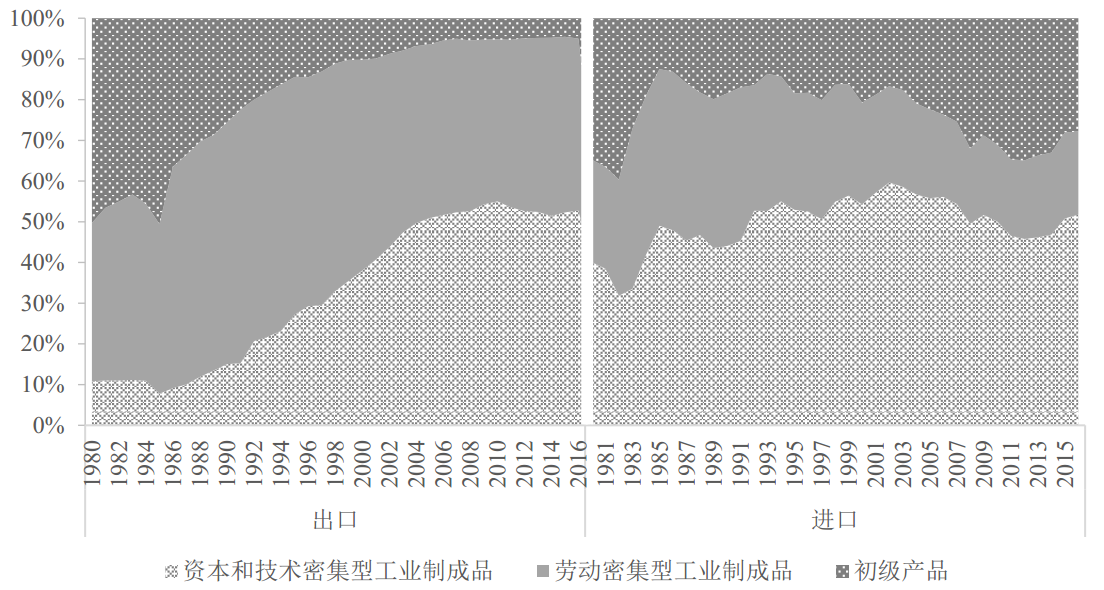
\includegraphics[scale=0.5]{fig/gravity/china2}
\end{frame}

\begin{frame}{中国进出口流向的变化(1998-2016 年)}
\centering 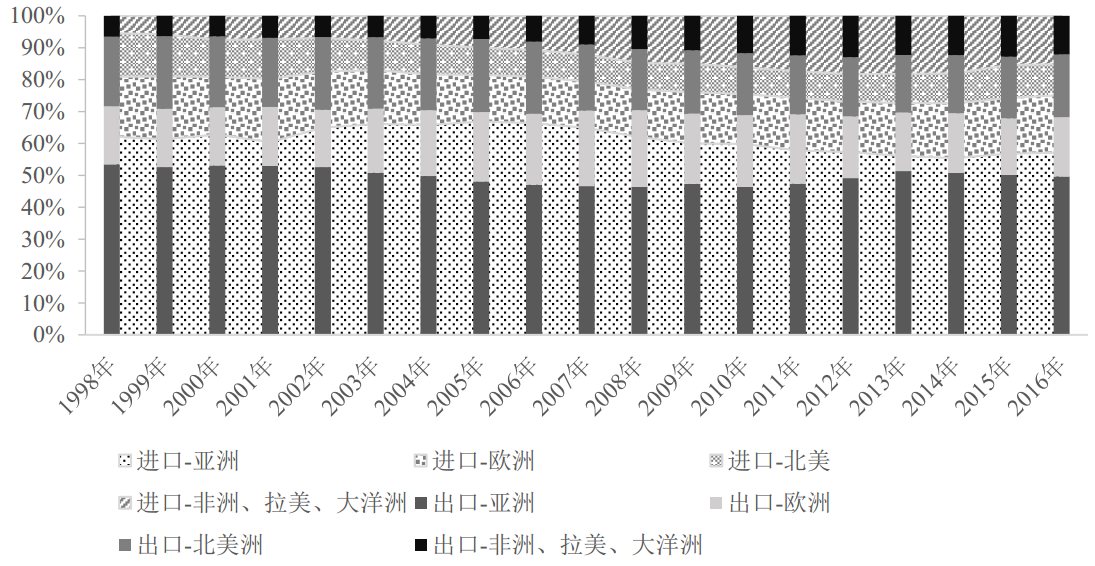
\includegraphics[scale=0.55]{fig/gravity/china3}
\end{frame}

\begin{frame}{全球直接投资中的中国}
\centering 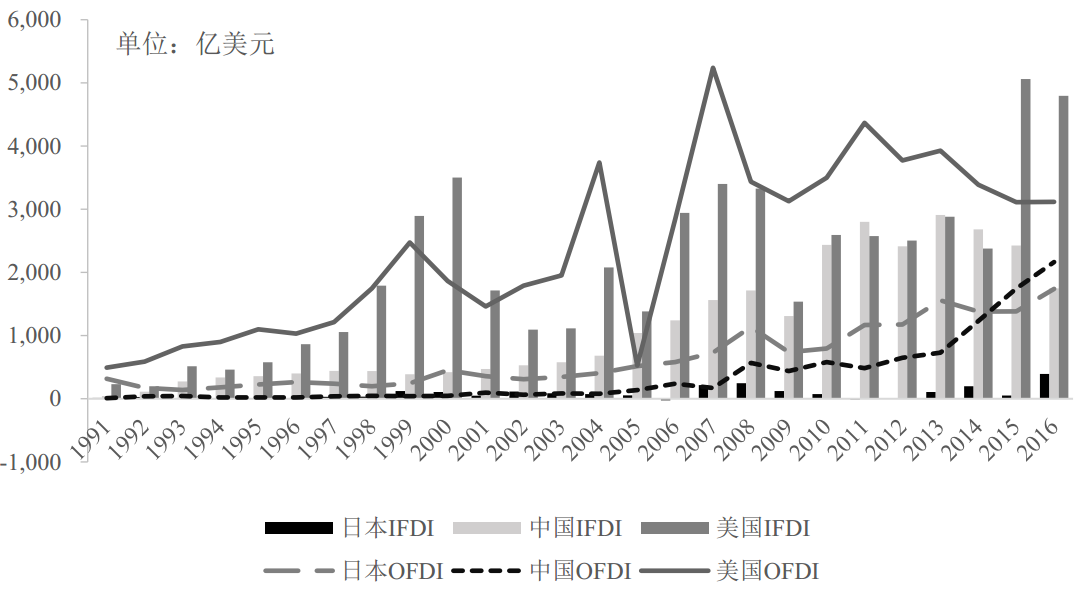
\includegraphics[scale=0.5]{fig/gravity/china4}
\end{frame}

\begin{frame}{中国受到的反倾销调查和措施}
\centering 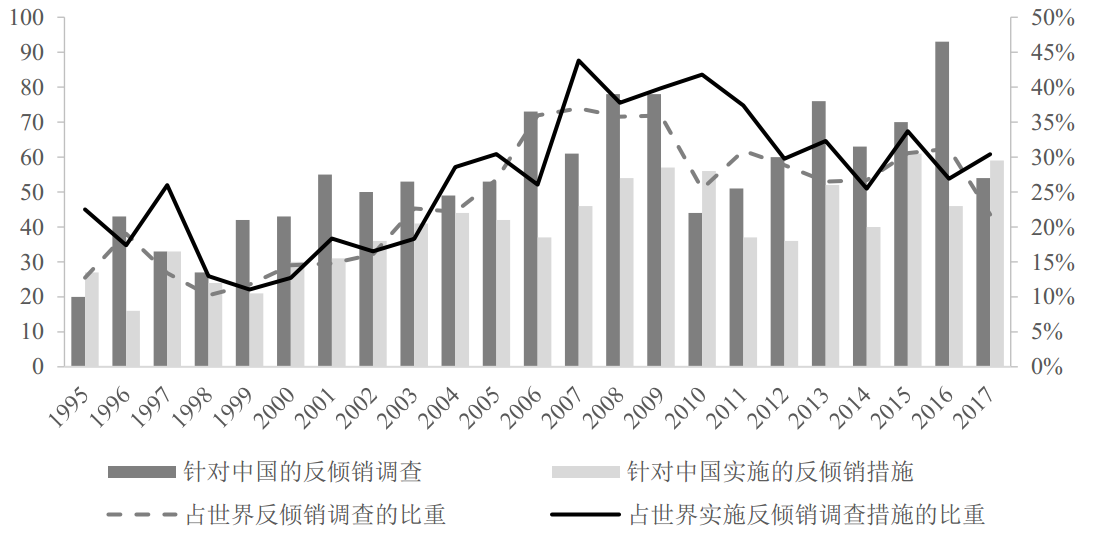
\includegraphics[scale=0.55]{fig/gravity/china5}
\end{frame}


\section{贸易背后的影响因素初探:以美国为例}

\begin{frame}{Main U.S. Trading Partners in 2012}


\begin{columns}[onlytextwidth]
	\begin{column}{0.60\textwidth}
		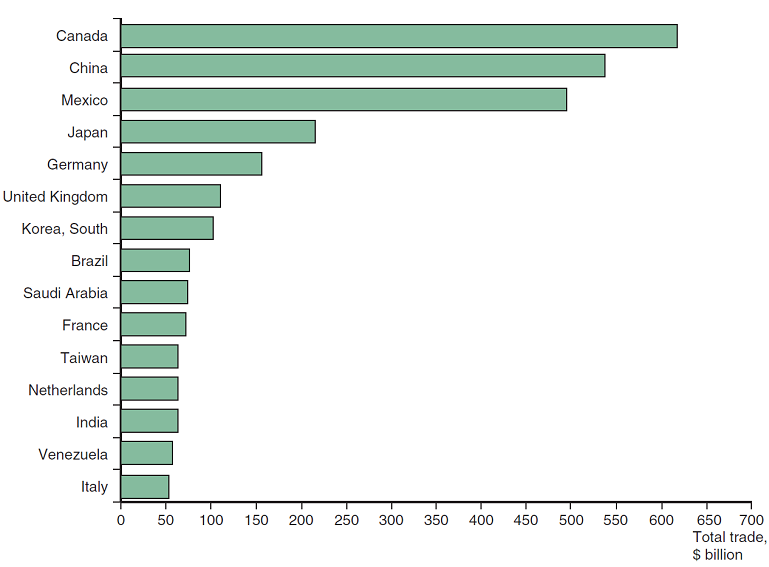
\includegraphics[width=\columnwidth]{fig/gravity/tra9}
		
		
	\end{column}
	\begin{column}{0.40\textwidth}
		
		
		\pause{}
		\begin{itemize}
			\item Geography and size are important determinants of bilateral trade flows
		\end{itemize}
		
		\pause{}
		\begin{itemize}
			\item 5 largest U.S. trading partners in 2012: Canada, China, Mexico, Japan
			and Germany 
		\end{itemize}
		
		\pause{}
		\begin{itemize}
			\item The largest 15 trading partners with the U.S. accounted for 69\% of
			the value of US trade in 2012
		\end{itemize}
		
	\end{column}
\end{columns}

\end{frame}

\begin{frame}{The Effect of Size on U.S.-EU Trade}


\begin{figure}


\centering{}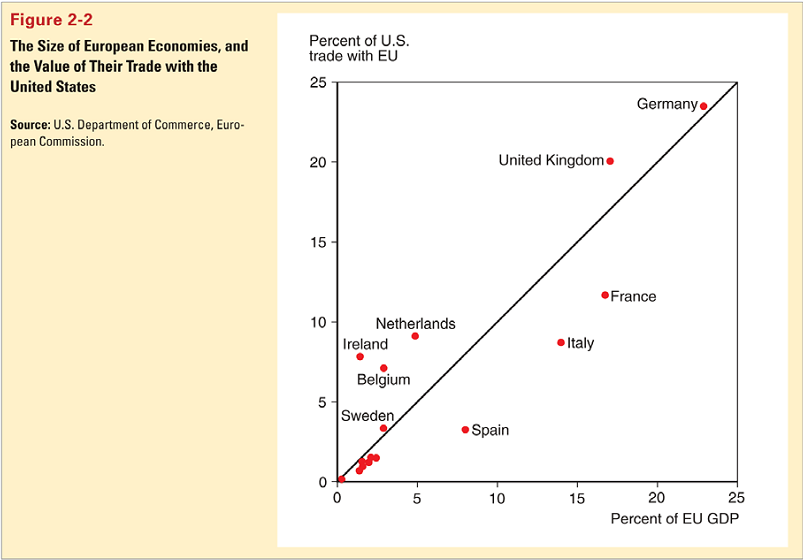
\includegraphics[width=8cm]{fig/gravity/tra10}
\end{figure}

\begin{itemize}
\item Note that the slope is close to 1 
\end{itemize}
\end{frame}

\begin{frame}{Towards A Quantitative Equation}

\begin{itemize}
\item Suppose that the fraction of income that any foreign country (say
U.K.) spends on U.S. goods is equal to the share of U.S. goods in
world spending… 
\item … which is equal to the U.S. share of world GDP 
\item The total spending of consumers from any given country (say U.K.)
is equal to that country’s GDP
\item So exports from U.S. to U.K are equal to:
\[
X^{US,UK}=\frac{GDP^{US}}{GDP^{World}}\times GDP^{UK}
\]

\end{itemize}
\end{frame}

\begin{frame}{Distance Matters}


\begin{columns}[onlytextwidth]
\begin{column}{0.4\textwidth}
\begin{itemize}
\item It makes intuitive sense that distance between markets will reduce
trade flows 
\item Directly through higher costs of transports 
\item Indirectly through less personal contact and communication
\end{itemize}

\end{column}
\begin{column}{0.6\textwidth}
\centering 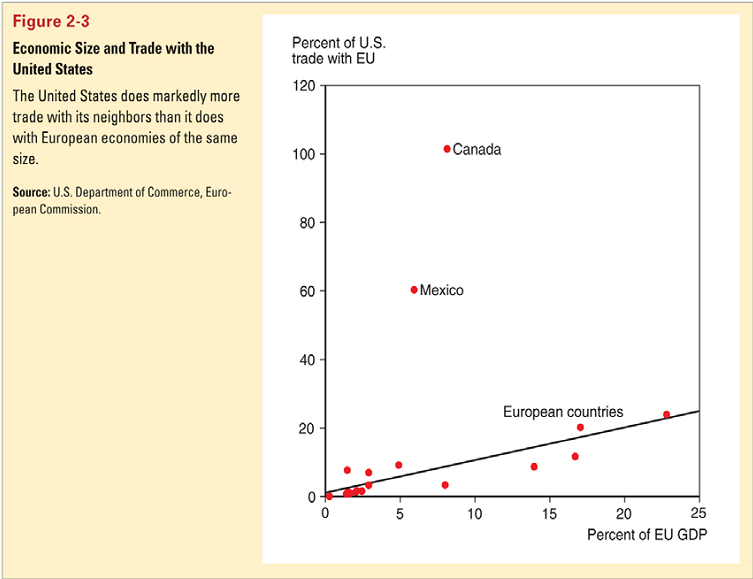
\includegraphics[width=0.8\columnwidth]{fig/gravity/tra11}
\end{column}
\end{columns}

\end{frame}



\section{How is the Trade Volume determinated: the Gravity Model }


\subsection{The Simplest Gravity Model}
\begin{frame}{The Gravity Equation: Benchmark}

\begin{itemize}
\item In its basic form, the gravity model assumes that only size and distance
are important for trade in the following way:
\end{itemize}

\begin{center}
$T{}^{ij}=\frac{AY^{i}Y^{j}}{D^{ij}}$
\par\end{center}
\begin{itemize}
\item where

\begin{itemize}
\item $T{}^{ij}$is the value of trade between country $i$ and country
$j$
\item $A$ is a constant 
\item $Y^{i}$is the GDP of country $i$ 
\item $Y^{j}$is the GDP of country $j$ 
\item $D^{ij}$is the distance between country $i$ and country $j$ 
\end{itemize}
\item Analogy to Newton’s law of gravitation 

\begin{itemize}
\item Gravitational attraction is proportional to the product of masses
and inversely proportional to the square of distance 
\end{itemize}
\end{itemize}
\end{frame}

\begin{frame}{The Gravity Equation: an Extended Version}

\begin{itemize}
\item The assumptions needed to get proportionality of GDPs are strong 
\item A more general form is
\[
T^{ij}=A\text{·}(Y^{i})^{a}\text{·}(Y^{j})^{b}/(D^{ij})^{c}
\]
\[
lnT^{ij}=lnA+alnY^{i}+blnY^{j}-clnD^{ij}
\]

\item where $a$, $b$, and $c$ are allowed to differ from 1 
\item The gravity equation is very easy to run (widely available data online
– e.g., Andrew K. Rose’s website) 
\item Perhaps surprisingly, the gravity model works fairly well in predicting
actual trade flows 
\item Coefficients $a$, $b$ and $c$ are all close to 1 
\item Typical $R{}^{2}$≈80\%
\end{itemize}
\end{frame}

\begin{frame}{Embellishing the Gravity Equation}

\begin{itemize}
\item Obviously, there are many other determinants of bilateral trade flows 
\item The evidence confirms the “statistical significance” of: 

\begin{itemize}
\item sharing a common border (beyond the effect of distance); 
\item sharing a common language or colonial links; 
\item having signed a free trade agreement; 
\item having cultural ties
\item Business networks
\end{itemize}
\item useful resource of the above infromation: \href{http://www.cepii.org}{CEPII gravity database}
\end{itemize}
\end{frame}

\begin{frame}{经济学中的孤儿:The Theoritical Fundation of GE}

\begin{itemize}
\item The gravity model was popular in the 1960’s by Tingbergen(1962) initially,
because it could account for empirical regularities of world trade
that were not explained by traditional theories. 
\item However, most of its first economic applications were empirical studies,
without any serious attempt to justify the model theoretically. 
\item The development of theories of intra-industry trade made it possible
to give theoretical foundations to this “orphan” equation. 
\item There is today a wealth of economic justifications for this equation:

\begin{itemize}
\item general equilibrium model with pure and perfect competition and differentiated
products
\item models with monopolistic competition
\item the Heckscher-Ohlin’s model
\end{itemize}
\item the gravity equation can by justified by \textcolor{red}{almost any
model} in which countries specialize in the production of differentiated
goods.
\end{itemize}
\end{frame}



\subsection{Border Effect in GE}
\begin{frame}{Border Effects}

\begin{itemize}
\item Other things equal, countries trade more with their neighbors
\item First Raised by McCallum(AER, 1995)
\item But borders significantly impede trade flows (relative to intra-national
trade flows) 
\end{itemize}

\begin{figure}


\begin{centering}
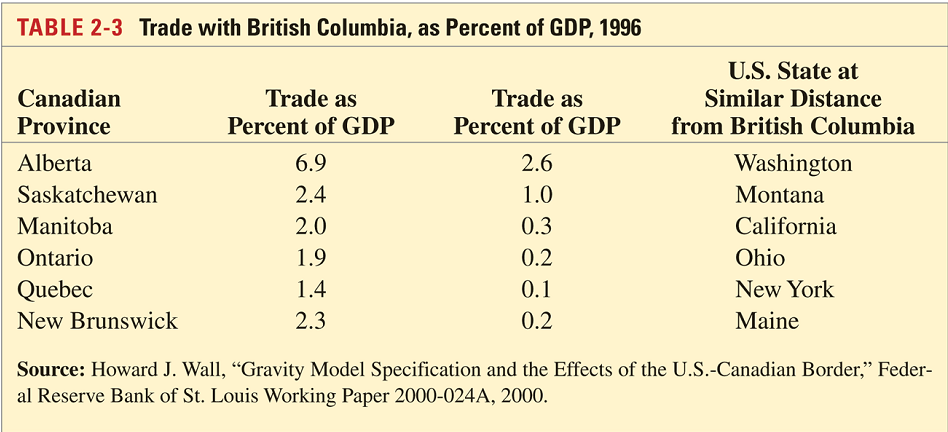
\includegraphics[width=8cm]{fig/gravity/tra12}
\par\end{centering}

\end{figure}


\end{frame}

\begin{frame}{Border Effects}


\begin{figure}
\begin{centering}
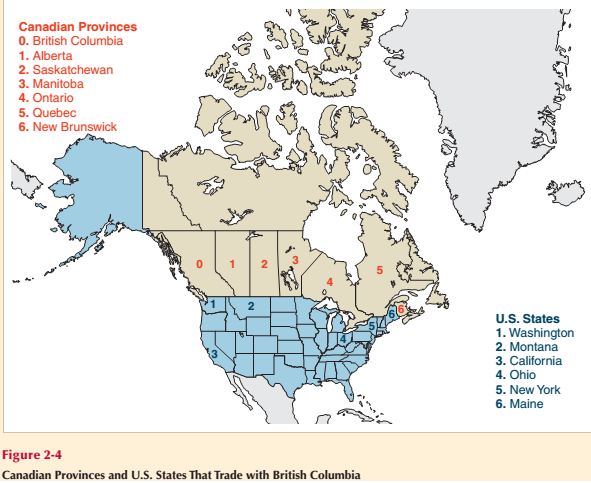
\includegraphics[width=7cm]{fig/gravity/tra13}
\par\end{centering}

\end{figure}

\begin{itemize}
\item Estimates suggest that the border between the U.S. and Canada is around
2000 miles wide
\end{itemize}
\end{frame}

\begin{frame}{Estimating border effects}


The basic gravity equation with BE is
\begin{equation*} 
\ln x^{ij}=\alpha _{0}+\alpha _{1}\ln y^{i}+\alpha _{2}\ln y^{j}+\alpha _{3}\ln d^{ij}+\alpha _{4} \delta^{ij}+u_{ij}
\end{equation*}% 
where% 
\begin{equation*} 
\delta ^{ij}=\left\{ 
\begin{array}{ll} 
1 & \text{if }i\text{ and }j\text{ are two Canadian provinces} \\ 
0 & \text{if }i\text{ is a Can. province and }j\text{ a US state or vice versa.}%
It makes intuitive sense that distance between markets will reduce trade flows 
Directly through higher costs of transports 
Indirectly through less personal contact and communication


\end{array}% 
\right. 
\end{equation*}% 
Estimated BE: Let $\widehat{x}_{can}^{ij}$ be the estimated trade between 
two Canadian provinces and $\widehat{x}^{ij}$ the estimated trade between a 
Canadian province and a US state. 
\begin{equation*} 
\ln \widehat{x}_{can}^{ij}-\ln \widehat{x}^{ij}=\widehat{\alpha }_{4} 
\end{equation*}% 
so BE is% 
\begin{equation*} 
\frac{\widehat{x}_{can}^{ij}}{\widehat{x}^{ij}}=e^{\widehat{\alpha }_{4}}; 
\end{equation*}% 
$\widehat{\alpha }_{4}=3.09$ implies a BE of 26.97. Suspiciously large!
\end{frame}


\begin{frame}{引力方程的后续进展} 
  \begin{itemize}
  	\item McCallum(1995)的结果出乎经济学家的预料推动了该领域的进展
  	\item Anderson and Wincoop(2003)提出一种猜想:由于美国加拿大经济规模悬殊,故而可能导致估计错误,因为贸易中存在“多边引力”
  	\item 在Melitz(2003)之后,国际贸易研究开始全面向微观领域进发,推动了引力方程向企业层贸易延伸
  		\begin{itemize}
  			\item Helpman, Melitz and Robinstein(2008)基于异质企业贸易模型,引入一个考虑企业自主选择出口目的地因素的\emph{广义引力等式Generalized Gravity Equation},并将贸易流量分解为Intensive and Extensive两个Margins.
  			\item Chaney(2011)做出一个更为大胆的尝试,考虑贸易网络与初创不成熟贸易网络两分的情形,引出了\emph{企业间的匹配问题},该模型被称为\textbf{考虑匹配摩擦约束下的贸易模型Model of Trade Subject to Matching Frictions}
  		\end{itemize}
  \end{itemize}
\end{frame}

\begin{frame}{总结}
Today's Takeways
\end{frame}
\end{document}